\documentclass[conference]{IEEEtran}
\IEEEoverridecommandlockouts
\usepackage[T1]{fontenc}
\usepackage{mathptmx}
\usepackage{graphicx}
\usepackage{booktabs}
\usepackage{multirow}
\usepackage{array}
\usepackage{tikz}
\usetikzlibrary{positioning,arrows.meta,fit,calc}
\usepackage{cite}
\usepackage{xcolor}
\usepackage{xurl}
\usepackage[hidelinks]{hyperref}
\graphicspath{{figures/}}
\newcommand{\clipA}{Clip~A}
\renewcommand{\arraystretch}{1.08}
\raggedbottom

\begin{document}

\title{Emotion Recognition Using\\Explainable Machine Learning\\[4pt]
{\large Do Accuracy and SHAP Explanations Survive a Change of Speech Corpus?}}

\author{
\IEEEauthorblockN{Pranav Sajith}
\IEEEauthorblockA{BL.SC.U4CSE24039 \\
\textit{Dept. of Computer Science and Engg.} \\
\textit{Amrita School of Computing} \\
\textit{Amrita Vishwa Vidyapeetham} \\
Bengaluru, India}
\and
\IEEEauthorblockN{Piriya Shreyash Shanmukh}
\IEEEauthorblockA{BL.SC.U4CSE24037 \\
\textit{Dept. of Computer Science and Engg.} \\
\textit{Amrita School of Computing} \\
\textit{Amrita Vishwa Vidyapeetham} \\
Bengaluru, India}
\and
\IEEEauthorblockN{Praveen Raj}
\IEEEauthorblockA{BL.SC.U4CSE24040 \\
\textit{Dept. of Computer Science and Engg.} \\
\textit{Amrita School of Computing} \\
\textit{Amrita Vishwa Vidyapeetham} \\
Bengaluru, India}
}

\maketitle

\begin{abstract}
Most speech emotion recognition (SER) results are reported on the same dataset the model was trained on, often with the same speakers on both sides of the split, and the explanations that come with them are seldom checked. In this project we build a six-class SER system (neutral, happy, sad, angry, fearful, disgust) on two acted English corpora, RAVDESS (24 actors, 1{,}056 clips) and CREMA-D (91 actors, 7{,}442 clips), and evaluate it only on speakers it has never heard. Every clip is described in two ways: by the 88 named eGeMAPS acoustic parameters and by a 768-number embedding from a frozen WavLM base-plus encoder. We compare logistic regression, an RBF-kernel SVM, LightGBM and a small neural network on each representation and on their combination, using nested, speaker-grouped cross-validation. Logistic regression on the combined features works best: 82.2\% unweighted average recall (UAR) on RAVDESS and 74.1\% on CREMA-D, where chance is 16.7\%, with a calibration error of about 0.02. Splitting the data randomly instead would have added up to 9.3 points on RAVDESS. A second linear model on the named features gives an exact SHAP explanation for every prediction. We also report train, validation and test scores for all 24 models, class-separability, PCA and correlation analyses, and two transfer experiments. Moving a model to the other corpus costs 20 to 35 points, and its SHAP rankings change more between corpora (Spearman 0.50, or 0.10 for WavLM) than between resamples of the same corpus (0.78 and 0.68). A Streamlit app runs the saved models and shows the reasons behind each answer.
\end{abstract}

\begin{IEEEkeywords}
speech emotion recognition, explainable AI, SHAP, eGeMAPS, WavLM, speaker independence, cross-corpus evaluation
\end{IEEEkeywords}

%=====================================================================
\section{Introduction}
%=====================================================================
The same sentence can sound calm, cheerful or furious depending on how it is spoken. Loudness, pitch, speaking rate and the quality of the voice all shift with the speaker's state, and speech emotion recognition tries to read the emotion from those cues. Typical uses include flagging frustrated callers in a contact centre, educational and assistive tools, and voice assistants that react to the user's tone.

Two developments have shaped recent SER research. Self-supervised speech encoders such as wav2vec~2.0 and WavLM now give general-purpose embeddings that beat hand-crafted acoustic features once a simple classifier is put on top~\cite{pepino,dixit,pastor}. At the same time, explainable AI (XAI) methods, SHAP~\cite{shap} above all, are being used to show which acoustic properties a model depends on~\cite{dixit,nfissi}. In almost every case, though, both are evaluated inside a single corpus.

This leaves three practical gaps. If the same speaker shows up in the training and the test data, a model can score well simply by recognising the voice, so the reported accuracy is too optimistic. A model that does well on one recording setup may do badly on another. And an explanation worked out once, on one dataset, may not describe what the model does anywhere else. We look at all three using two public English corpora.

\textbf{Running example.} To make each step concrete, one recording is followed through the paper. \clipA{} is the RAVDESS file \texttt{03-01-05-02-01-02-09.wav}: actor~9 says ``Kids are talking by the door'' with strong anger, in a 3.77\,s recording at 48\,kHz. Actor~9 is in test fold~0, so no model that scores \clipA{} has heard his voice during training.

\textbf{Contributions.} (i)~A speaker-independent comparison of eGeMAPS, WavLM and combined features with four classifiers on RAVDESS and CREMA-D, with train, validation and test scores. (ii)~Class-separability, dimensionality and correlation analyses of both feature sets. (iii)~Exact SHAP explanations for every prediction, checked against permutation importance. (iv)~Measurements of how much accuracy and SHAP rankings move across resamples, speaker groups and corpora. (v)~A working application built on the saved models.

%=====================================================================
\section{Literature Survey}
%=====================================================================
Table~\ref{tab:lit} lists the fifteen papers that shaped the project. We group them by what they contributed.

\emph{Datasets.} RAVDESS~\cite{ravdess} and CREMA-D~\cite{cremad} both use actors performing intended emotions. When listeners heard the audio alone, they picked the intended emotion for 63\% of RAVDESS speech files and only 40.9\% of CREMA-D clips. Vocal emotion is therefore ambiguous even for human listeners, which sets a realistic ceiling for any model.

\emph{Features and models.} eGeMAPS~\cite{egemaps} is a small, standard set of 88 acoustic parameters agreed on by voice and emotion researchers. Its authors found that it did as well as a far larger feature set for arousal, and suggested (without testing it) that compact features might generalise better between databases. WavLM~\cite{wavlm} is a self-supervised Transformer; the base-plus model we use was pre-trained on 94{,}000 hours of speech. Pepino \emph{et al.}~\cite{pepino} reached 84.3\% UAR on RAVDESS with wav2vec~2.0 embeddings against 57.0\% with eGeMAPS, and found that the middle layers hold the most emotion information. Ko{\l}odziej \emph{et al.}~\cite{kolodziej} and Kaloga and Kodrasi~\cite{kaloga} compared hand-crafted features and classical classifiers under speaker-independent testing.

\emph{Explainability.} SHAP~\cite{shap} splits a prediction into additive contributions, one per feature. Dixit \emph{et al.}~\cite{dixit} combined SHAP with probing to relate WavLM embeddings to eGeMAPS and found energy features to be the most informative. Nfissi \emph{et al.}~\cite{nfissi} used SHAP to pick features, and Nasr \emph{et al.}~\cite{nasr} checked whether saliency maps agree with the acoustic cues experts look for.

\emph{Cross-corpus generalisation.} Schuller \emph{et al.}~\cite{schuller} showed early on that accuracy across corpora is far below accuracy within one, and that normalising each corpus separately helps. Pastor \emph{et al.}~\cite{pastor} found that adding CREMA-D to the training data can even hurt results on another corpus, and two recent benchmarks~\cite{phukan,ibrahim} compare pre-trained encoders across several corpora.

\begin{table*}[!t]
\centering
\caption{Literature survey: models, metrics and reported results (numbers from each paper; protocols differ, so they are not directly comparable)}
\label{tab:lit}
\footnotesize
\begin{tabular}{@{}p{3.1cm}p{4.7cm}p{3.6cm}p{5.2cm}@{}}
\toprule
\textbf{Paper} & \textbf{Data and model} & \textbf{Metric / protocol} & \textbf{Reported result} \\
\midrule
RAVDESS~\cite{ravdess}, 2018 & 24 actors; 247 raters, 10 ratings per file & proportion correct, kappa & 63\% human accuracy, audio-only speech \\
CREMA-D~\cite{cremad}, 2014 & 91 actors; 2{,}443 crowd raters & recognition rate per modality & 40.9\% audio-only, 63.6\% audio-visual \\
eGeMAPS~\cite{egemaps}, 2016 & 62/88 parameters, linear SVM, 6 corpora & UAR, leave-speaker-group-out & 79.7\% binary arousal (larger set 78.0\%) \\
WavLM~\cite{wavlm}, 2022 & self-supervised Transformer & SUPERB benchmark tasks & base-plus emotion task 68.65\% \\
SHAP~\cite{shap}, 2017 & Kernel and Deep SHAP & axioms, user study & unique additive attribution with all three axioms \\
Pepino \emph{et al.}~\cite{pepino}, 2021 & wav2vec 2.0 layers, dense/LSTM heads & UAR, actor split & 84.3\% RAVDESS vs 57.0\% eGeMAPS \\
Dixit \emph{et al.}~\cite{dixit}, 2024 & WavLM Large + eGeMAPS, LogReg, probes & F1, speaker-independent CV & energy group most informative \\
Ko{\l}odziej \emph{et al.}~\cite{kolodziej}, 2026 & 107 features vs fine-tuned WavLM & balanced accuracy, LOSO & 0.727 WavLM vs 0.627 features \\
Kaloga, Kodrasi~\cite{kaloga}, 2025 & ComParE, six classifiers, 6 corpora & UAR, 3 runs & 62.5\% average UAR \\
Nfissi \emph{et al.}~\cite{nfissi}, 2023 & SHAP-guided feature boosting, trees & accuracy, F1 & 98.7\% on TESS (two speakers) \\
Pastor \emph{et al.}~\cite{pastor}, 2023 & HuBERT/WavLM, cross-corpus training & UAR, speaker-disjoint & adding CREMA-D: IEMOCAP 66.90 $\to$ 65.06\% \\
Phukan \emph{et al.}~\cite{phukan}, 2025 & 8 pre-trained encoders, 5 corpora & accuracy, macro-F1 & CREMA-D: 79.7\% best encoder, 71.4\% WavLM \\
Ibrahim \emph{et al.}~\cite{ibrahim}, 2024 & Whisper fine-tuned, 11 corpora & weighted accuracy & 87.5\% RAVDESS, 4 classes \\
Schuller \emph{et al.}~\cite{schuller}, 2010 & SVM, 6 corpora, 409 experiments & UAR, WAR & speaker normalisation best; cross $\ll$ within \\
Nasr \emph{et al.}~\cite{nasr}, 2025 & spectrogram ResNet, occlusion, CRP & accuracy, plausibility & 0.63 CREMA-D accuracy \\
\bottomrule
\end{tabular}
\end{table*}

\textbf{Research gap.} From these papers it is clear that embeddings beat named features inside a corpus and that accuracy falls sharply across corpora. What they do not tell us is whether SHAP explanations stay the same when the training sample, the speakers or the corpus change, or whether the explanations agree with a second, independent method. We did not find a study that measures SHAP stability for RAVDESS and CREMA-D in both directions. Our search was not exhaustive, so we call this an underexplored question rather than a new one.

%=====================================================================
\section{Problem Statement and Objectives}
%=====================================================================
\textbf{Problem statement.} Build a six-class speech emotion recognition system that is tested only on speakers it has not heard, explains each prediction in terms of named voice properties, and measures whether its accuracy and explanations still hold when it is moved to a different corpus.

\textbf{Research question.} If a model trained on one acted English corpus is used on another, do its accuracy and its SHAP explanations hold up? We wrote down four hypotheses before running any experiment. \textbf{H0}: random splits inflate accuracy, and more so for the corpus with fewer speakers. \textbf{H1}: WavLM is better within a corpus but loses relatively more than eGeMAPS across corpora. \textbf{H2}: SHAP rankings are most stable across resamples, less across speaker groups, least across corpora, and always above a random baseline. \textbf{H3}: a ``stable core'' of features transfers better than the usual top-$k$ features.

\textbf{Objectives.} O1: prepare and explore both corpora, with folds grouped by speaker. O2: compare three feature sets and four classifiers fairly using nested cross-validation. O3: explain every prediction and check the explanations. O4: test transfer between the corpora and the stability of the explanations. O5: save the trained models and build a working demo.

%=====================================================================
\section{Data Exploration and Preprocessing}
%=====================================================================
\subsection{Datasets}
Table~\ref{tab:data} compares the two corpora. We keep the six emotions they have in common and drop the RAVDESS \emph{calm} and \emph{surprised} clips (384 files). Neutral is the smallest class in both: 96 clips against 192 for the other emotions in RAVDESS, and 1{,}087 against 1{,}271 in CREMA-D. For that reason UAR is our main metric and every classifier uses balanced class weights. All files could be read; five RAVDESS files turned out to be stereo. CREMA-D also provides listener ratings, which are informative about label quality. The listeners' majority vote on the audio matches the intended emotion for only 41.6\% of clips, ranging from 95.7\% for neutral down to 16.4\% for sad, and 847 clips meant to be sad were heard as neutral. Our model's recall per emotion follows the same order as the listeners' agreement (Spearman 0.60), and its UAR is 84.3\% on clips where listeners agreed with the label but 67.2\% on the rest. Part of the CREMA-D error is therefore noise in the labels rather than a failure of the model.

\begin{table}[!t]
\centering
\caption{The two corpora}
\label{tab:data}
\footnotesize
\setlength{\tabcolsep}{3pt}
\begin{tabular}{@{}lll@{}}
\toprule
 & \textbf{RAVDESS}~\cite{ravdess} & \textbf{CREMA-D}~\cite{cremad} \\
\midrule
Speakers & 24 (12 F, 12 M), 21--33 y & 91 (43 F, 48 M), 20--74 y \\
Sentences & 2 & 12 \\
Clips used & 1{,}056 of 1{,}440 & 7{,}442 \\
Audio & 48 kHz, studio & 16 kHz, varied \\
Mean length & 3.70 s & 2.54 s \\
Human acc. (audio) & 63\% & 40.9\% \\
Licence & CC BY-NC-SA 4.0 & ODbL 1.0 \\
\bottomrule
\end{tabular}
\end{table}

\textbf{Splits.} Each corpus is split into five folds with \texttt{StratifiedGroupKFold} (seed 42), grouped by speaker and balanced for emotion and gender. We checked in code that no speaker appears in more than one fold.

\subsection{Preprocessing}
Every clip is mixed down to mono, resampled to 16\,kHz with exact polyphase filtering, and trimmed at both ends. Anything more than 30\,dB below the loudest point of the clip is treated as silence, but a clip is never cut below 0.25\,s. We deliberately do not normalise the volume, because loudness is one of the strongest emotion cues. Trimming roughly halved the RAVDESS clips, from 3.70\,s to 1.90\,s on average. Features are standardised and clipped to $\pm$5 standard deviations inside each model pipeline, using statistics from the training data only.

For \clipA{}, resampling turns 180{,}981 samples at 48\,kHz into 60{,}327 samples at 16\,kHz. Trimming keeps samples 15{,}360 to 45{,}568, which is 30{,}208 samples or 1.89\,s of speech (Fig.~\ref{fig:pre}).

\begin{figure}[!t]
\centering
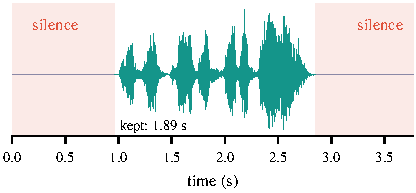
\includegraphics[width=\columnwidth]{fig_preprocessing}
\caption{\clipA{} after resampling to 16\,kHz. The shaded edges lie more than 30\,dB below the peak and are removed as silence; the teal part (1.89\,s) is what the models receive.}
\label{fig:pre}
\end{figure}

%=====================================================================
\section{Proposed Methodology}
%=====================================================================
\subsection{System overview}
Fig.~\ref{fig:block} gives the overall design. After cleaning, each clip goes through two feature extractors. The \emph{predictor} classifies the combined features. The \emph{explainer} sees only the named eGeMAPS features, so every SHAP value it produces refers to something measurable about the voice.

\begin{figure*}[!t]
\centering
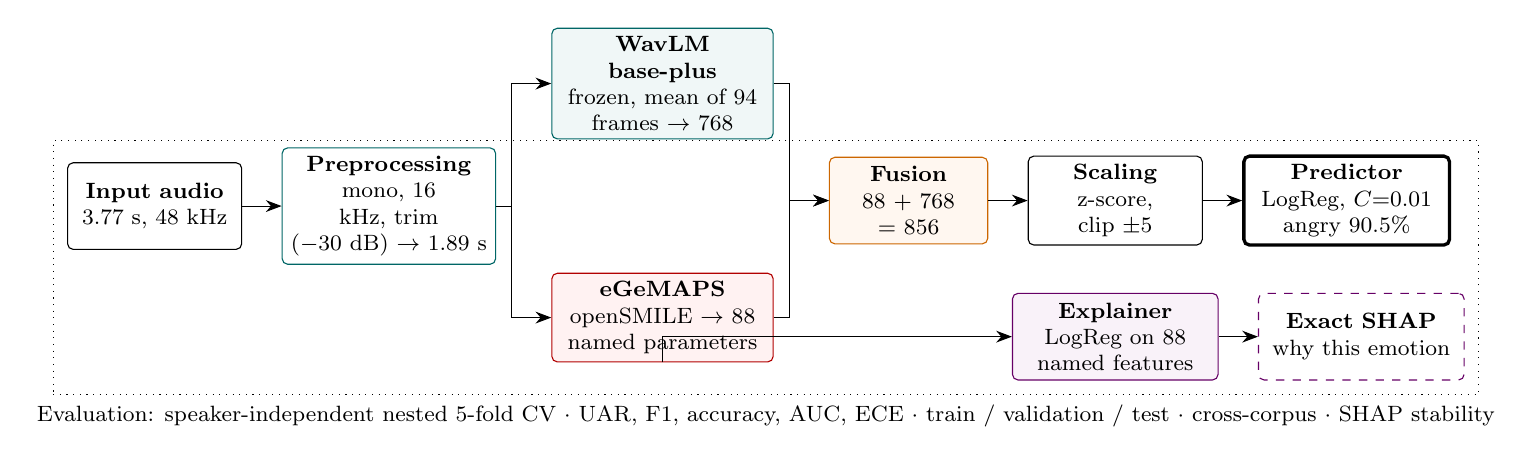
\begin{tikzpicture}[font=\footnotesize, node distance=4mm and 5mm,
  box/.style={draw, rounded corners=2pt, align=center, minimum height=11mm, inner sep=3pt, text width=#1},
  box/.default=22mm, >={Stealth[length=2mm]}]
\node[box=20mm] (in) {\textbf{Input audio}\\3.77 s, 48 kHz};
\node[box=25mm, right=of in, draw=teal!80!black] (pre) {\textbf{Preprocessing}\\mono, 16 kHz, trim\\(${-}30$ dB) $\to$ 1.89 s};
\node[box=26mm, above right=1mm and 7mm of pre, draw=teal!80!black, fill=teal!6] (wl) {\textbf{WavLM base-plus}\\frozen, mean of 94\\frames $\to$ 768};
\node[box=26mm, below right=1mm and 7mm of pre, draw=red!70!black, fill=red!5] (eg) {\textbf{eGeMAPS}\\openSMILE $\to$ 88\\named parameters};
\node[box=18mm, right=7mm of $(wl.east)!0.5!(eg.east)$, draw=orange!80!black, fill=orange!6] (fu) {\textbf{Fusion}\\88 + 768\\= 856};
\node[box=20mm, right=of fu] (sc) {\textbf{Scaling}\\z-score,\\clip $\pm$5};
\node[box=24mm, right=of sc, line width=1.2pt] (pr) {\textbf{Predictor}\\LogReg, $C{=}0.01$\\angry 90.5\%};
\node[box=24mm, below=6mm of sc, draw=violet!80!black, fill=violet!5] (ex) {\textbf{Explainer}\\LogReg on 88\\named features};
\node[box=24mm, right=of ex, dashed, draw=violet!80!black] (sh) {\textbf{Exact SHAP}\\why this emotion};
\draw[->] (in) -- (pre);
\draw[->] (pre.east) -- ++(2mm,0) |- (wl.west);
\draw[->] (pre.east) -- ++(2mm,0) |- (eg.west);
\draw[->] (wl.east) -- ++(2mm,0) |- (fu.west);
\draw[->] (eg.east) -- ++(2mm,0) |- (fu.west);
\draw[->] (fu) -- (sc); \draw[->] (sc) -- (pr);
\draw[->] (eg.south) |- (ex.west);
\draw[->] (ex) -- (sh);
\node[draw, dotted, fit=(in)(pr)(sh), inner sep=5pt, label={[font=\footnotesize]below:Evaluation: speaker-independent nested 5-fold CV $\cdot$ UAR, F1, accuracy, AUC, ECE $\cdot$ train / validation / test $\cdot$ cross-corpus $\cdot$ SHAP stability}] {};
\end{tikzpicture}
\caption{Block diagram of the proposed system, with the values for \clipA{}.}
\label{fig:block}
\end{figure*}

\subsection{Feature extraction}
\textbf{eGeMAPS.} The openSMILE toolkit measures 25 low-level descriptors every 10\,ms, including pitch, jitter, shimmer, loudness, harmonics-to-noise ratio, formants, spectral slopes and balance, MFCC 1--4 and spectral flux. These are then summarised over the whole clip with means, coefficients of variation, percentiles and slopes, together with a few temporal rates. The result is 88 named parameters in four groups: energy (15), frequency (24), spectral (43) and temporal (6)~\cite{egemaps,dixit}. As an example, \clipA{} has a mean loudness of 1.21, while the training mean is 0.417 with a standard deviation of 0.387. Its standardised value is $z = (1.21 - 0.417)/0.387 = +2.05$, which makes it louder than 94\% of all 8{,}498 clips.

\textbf{WavLM base-plus.} WavLM first passes the waveform through seven convolutional layers whose strides multiply to 320 samples, giving one 768-dimensional frame every 20\,ms. Twelve Transformer layers then let every frame attend to every other frame~\cite{wavlm}. We keep the encoder frozen and average each of its 13 layer outputs over time. For \clipA{}, 30{,}208 samples become 94 frames and finally 13$\times$768 numbers. Which layer to use is decided by inner cross-validation. The middle layers carry the most emotion information (Fig.~\ref{fig:layers}), which agrees with~\cite{pepino}, and the final model uses layer~7.

\begin{figure}[!t]
\centering
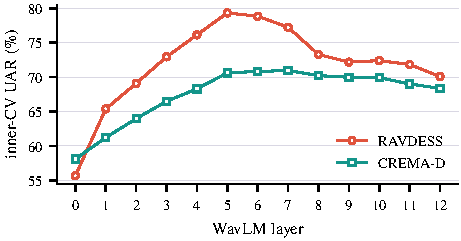
\includegraphics[width=\columnwidth]{fig_layers}
\caption{How much emotion information each WavLM layer holds: inner-CV UAR of a logistic regression on that layer's mean embedding.}
\label{fig:layers}
\end{figure}

\subsection{Dimensionality and correlation analysis}
Many of the 88 eGeMAPS parameters are strongly redundant. On RAVDESS, 134 of the 3{,}828 feature pairs have $|r|>0.8$ and 57 have $|r|>0.9$ (120 and 55 on CREMA-D), while the average $|r|$ is 0.23 (Fig.~\ref{fig:corr}). The strongest pairs are unsurprising: the relative amplitudes of F2 and F3 ($r=0.998$), mean and median pitch (0.995), and mean and 80th-percentile loudness (0.993). With principal component analysis (PCA), 37 of the 88 components keep 95\% of the eGeMAPS variance on RAVDESS (35 on CREMA-D). WavLM layer~7 needs 212 of its 768 components for the same 95\% (247 on CREMA-D), as shown in Fig.~\ref{fig:dim}a.

We then tested whether dimensionality reduction improves classification. PCA was fitted on the training folds only and followed by logistic regression (Fig.~\ref{fig:dim}b). For WavLM, 64 components are already enough for 80.2\% UAR on RAVDESS (81.2\% with all 768) and 71.0\% on CREMA-D (74.0\%), but below 16 components accuracy drops quickly. For eGeMAPS, every reduction lowered accuracy: RAVDESS UAR is 53.9\% with all 88 features and 50.2\% with 20 components. We therefore keep all the features and let L2 regularisation deal with the correlated inputs instead of throwing information away.

\begin{figure}[!t]
\centering
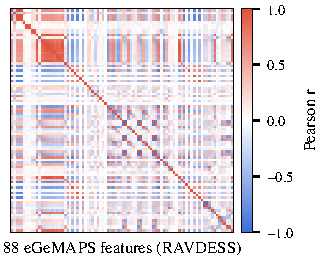
\includegraphics[width=0.78\columnwidth]{fig_correlation}
\caption{Pearson correlation between the 88 eGeMAPS features on RAVDESS (red positive, blue negative). The solid blocks are groups of redundant parameters such as loudness statistics and formant amplitudes.}
\label{fig:corr}
\end{figure}

\begin{figure*}[!t]
\centering
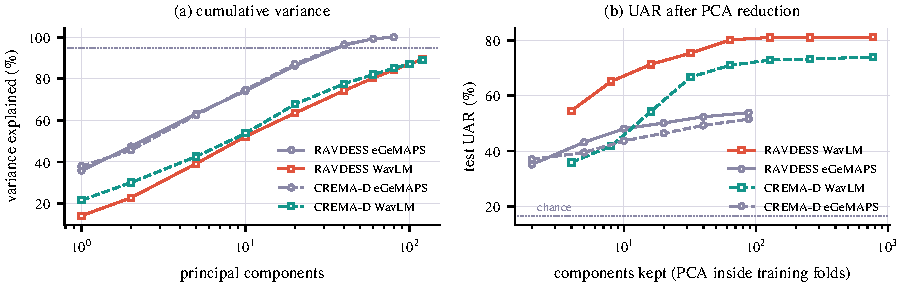
\includegraphics[width=0.92\textwidth]{fig_dimensionality}
\caption{Dimensionality analysis. (a) Cumulative variance explained by principal components; dotted line at 95\%. (b) Test UAR when only the first $k$ components are kept, with PCA fitted on training folds only.}
\label{fig:dim}
\end{figure*}

\subsection{Classifiers and training protocol}
We compare four classifiers implemented in scikit-learn and LightGBM; k-nearest neighbours was left out under a project rule. They are L2 logistic regression ($C\in\{0.01,0.1,1\}$), an RBF-kernel SVM ($C\in\{1,10\}$), LightGBM with 250 trees (minimum leaf size $\in\{10,30\}$), and a multilayer perceptron with 256 hidden units and early stopping ($\alpha\in\{10^{-3},10^{-1}\}$). Each one uses balanced class weights where the library allows it and is trained on eGeMAPS, WavLM and the combined features, which gives 24 models per corpus.

All evaluation is nested and speaker-independent. In each of the five outer folds, one fold is held out as the test set. On the other four folds, a 3-fold speaker-grouped inner cross-validation picks the hyperparameters and the WavLM layer; the inner score of the chosen setting is what we call the \emph{validation} score. The model is then refitted on those four folds (its score there is the \emph{training} score) and evaluated once on the held-out fold (the \emph{test} score). Our main metric is
\begin{equation}
\mathrm{UAR} = \frac{1}{6}\sum_{c=1}^{6}\frac{\mathrm{TP}_c}{\mathrm{TP}_c+\mathrm{FN}_c},
\end{equation}
the mean recall over the six emotions, so the smaller neutral class counts as much as any other. We also report macro-F1, accuracy, one-vs-rest ROC-AUC and the expected calibration error (ECE).

\subsection{Explainability}
For a linear model the SHAP values~\cite{shap} can be written down exactly. With standardised inputs $z$, weights $w_c$ for emotion $c$ and training mean $\bar z$, the contribution of feature $j$ is
\begin{equation}
\phi_{c,j} = w_{c,j}\,(z_j - \bar z_j), \qquad s_c = \beta_c + \sum_j \phi_{c,j},
\end{equation}
and the contributions add up exactly to the class score $s_c$ on the log-odds scale. Taking the difference $\phi_{a,j}-\phi_{b,j}$ answers the question ``why $a$ and not $b$?''. All explanations are computed out-of-fold, so each clip is explained by a model that never heard its speaker, and we compare them with permutation importance. To measure stability we take the Spearman correlation between the global importance rankings of two models trained on two resamples, two disjoint speaker groups or two corpora, and compare it with the correlation between random rankings.

%=====================================================================
\section{Implementation, Results and Discussion}
%=====================================================================
Everything is written in Python~3.11 using openSMILE, PyTorch/Transformers, scikit-learn, LightGBM and Streamlit, organised as seven notebooks and a \texttt{src/} package. The trained models are saved with joblib: the final model trained on all 115 speakers, a demo model trained without fold~0, and a variant made robust to microphone differences.

\subsection{Speaker leakage (H0)}
We first measured the effect of the split itself. Scoring the same logistic regression with a random clip-level split instead of speaker folds adds 9.3 points on RAVDESS with eGeMAPS (63.2 vs 53.9\%) and 7.8 points with WavLM (91.8 vs 84.0\%). On CREMA-D the gain is only 1.5 and 1.7 points. With just 24 speakers, a random split lets the model meet voices it has already heard. H0 is supported, and every result after this point uses speaker folds.

\subsection{Model comparison with train, validation and test scores}
Table~\ref{tab:tvt} lists all 24 models. WavLM is about 26 points better than eGeMAPS on RAVDESS and 22 points better on CREMA-D, and this holds in every fold. Combining the two adds 0.3 to 1.2 points for logistic regression. Logistic regression on the combined features is the best model on both corpora, with 82.2\% and 74.1\% test UAR. The training scores are far higher than the validation and test scores, most of all for LightGBM, which reaches 100\% on its training data but around 54\% on new speakers with eGeMAPS. The models fit their training speakers very closely, which is why only scores on unseen speakers are meaningful. Validation and test scores are within a few points of each other, which indicates that the settings selected on validation data were not tuned to the test speakers.

\begin{table*}[!t]
\centering
\caption{Train, validation and test scores of all 24 models (mean $\pm$ SD over 5 speaker-independent outer folds, \%). Train: refitted model on its own training folds; validation: inner 3-fold speaker-grouped CV of the chosen settings; test: unseen outer fold (the Phase 6 results; refitting with the same settings reproduced them within 1.0 points). Bold: best test UAR per corpus.}
\label{tab:tvt}
\footnotesize
\setlength{\tabcolsep}{4pt}
\begin{tabular}{@{}ll ccc cc @{\hspace{14pt}} ccc cc@{}}
\toprule
& & \multicolumn{5}{c}{\textbf{RAVDESS}} & \multicolumn{5}{c}{\textbf{CREMA-D}} \\
\cmidrule(lr){3-7}\cmidrule(l){8-12}
\textbf{Features} & \textbf{Model} & Train UAR & Val.\ UAR & Test UAR & Test F1 & Test Acc. & Train UAR & Val.\ UAR & Test UAR & Test F1 & Test Acc. \\
\midrule
eGeMAPS & LogReg & 73.1 & 52.7 $\pm$ 0.8 & 55.4 $\pm$ 2.6 & 53.5 & 54.1 & 56.0 & 51.3 $\pm$ 1.1 & 51.5 $\pm$ 3.3 & 50.7 & 51.2 \\
 & SVM (RBF) & 86.1 & 51.0 $\pm$ 1.1 & 52.4 $\pm$ 5.0 & 51.0 & 52.1 & 65.5 & 51.4 $\pm$ 0.9 & 52.8 $\pm$ 3.8 & 51.7 & 52.5 \\
 & LightGBM & 100.0 & 52.1 $\pm$ 3.2 & 53.9 $\pm$ 4.2 & 54.0 & 54.9 & 97.7 & 52.9 $\pm$ 1.3 & 53.8 $\pm$ 3.7 & 53.1 & 53.6 \\
 & MLP & 76.0 & 48.8 $\pm$ 1.9 & 51.4 $\pm$ 6.1 & 50.6 & 52.6 & 66.0 & 50.9 $\pm$ 0.8 & 52.0 $\pm$ 3.5 & 51.4 & 51.9 \\
\midrule
WavLM & LogReg & 99.7 & 80.4 $\pm$ 2.4 & 81.0 $\pm$ 5.9 & 80.4 & 80.6 & 85.4 & 73.7 $\pm$ 0.9 & 73.8 $\pm$ 1.9 & 73.6 & 73.5 \\
 & SVM (RBF) & 99.9 & 75.8 $\pm$ 2.4 & 78.5 $\pm$ 7.5 & 78.6 & 78.6 & 99.9 & 72.3 $\pm$ 1.0 & 73.4 $\pm$ 3.0 & 73.2 & 73.1 \\
 & LightGBM & 100.0 & 74.9 $\pm$ 2.7 & 76.8 $\pm$ 7.9 & 76.5 & 76.6 & 100.0 & 69.4 $\pm$ 1.2 & 70.3 $\pm$ 3.1 & 70.0 & 70.0 \\
 & MLP & 98.6 & 76.6 $\pm$ 2.8 & 78.6 $\pm$ 8.1 & 78.5 & 78.6 & 95.7 & 72.1 $\pm$ 1.0 & 72.5 $\pm$ 1.8 & 72.4 & 72.2 \\
\midrule
Fusion & LogReg & 99.7 & 80.6 $\pm$ 2.9 & \textbf{82.2 $\pm$ 5.1} & 81.6 & 81.9 & 86.6 & 73.6 $\pm$ 0.9 & \textbf{74.1 $\pm$ 2.2} & 73.9 & 73.8 \\
 & SVM (RBF) & 99.8 & 76.6 $\pm$ 2.4 & 78.8 $\pm$ 9.4 & 78.6 & 78.7 & 100.0 & 72.5 $\pm$ 1.3 & 73.4 $\pm$ 3.4 & 73.2 & 73.1 \\
 & LightGBM & 100.0 & 75.0 $\pm$ 3.4 & 76.3 $\pm$ 7.3 & 76.5 & 76.8 & 100.0 & 69.9 $\pm$ 1.8 & 70.2 $\pm$ 4.2 & 70.0 & 69.9 \\
 & MLP & 99.1 & 77.7 $\pm$ 2.9 & 81.3 $\pm$ 4.3 & 80.8 & 80.6 & 96.1 & 72.0 $\pm$ 1.2 & 73.1 $\pm$ 3.6 & 73.0 & 72.8 \\
\bottomrule
\end{tabular}
\end{table*}


\subsection{Per-emotion performance and calibration}
Table~\ref{tab:prf} and Fig.~\ref{fig:cm} look at the best model emotion by emotion. On RAVDESS, angry and disgust are the easiest (F1 0.89). Sad is the hardest emotion in both corpora and tends to absorb quiet deliveries: 14\% of fearful RAVDESS clips and 17\% of fearful CREMA-D clips end up labelled sad. Macro ROC-AUC is 0.968 on RAVDESS and 0.944 on CREMA-D, and the expected calibration error is 0.025 and 0.021. In other words, predictions made with 80\% confidence are correct about 80\% of the time. Happy and angry, the two loud emotions, are mixed up in roughly 5\% of clips in each direction.

\begin{table}[!t]
\centering
\caption{Precision / recall / F1 of the best model (LogReg, fusion), out-of-fold on unseen speakers}
\label{tab:prf}
\footnotesize
\begin{tabular}{@{}lcc@{}}
\toprule
\textbf{Emotion} & \textbf{RAVDESS} & \textbf{CREMA-D} \\
\midrule
neutral & 0.76 / 0.87 / 0.81 & 0.77 / 0.86 / 0.81 \\
happy & 0.84 / 0.76 / 0.80 & 0.78 / 0.76 / 0.77 \\
sad & 0.68 / 0.75 / 0.71 & 0.65 / 0.67 / 0.66 \\
angry & 0.89 / 0.90 / 0.89 & 0.84 / 0.83 / 0.83 \\
fearful & 0.83 / 0.79 / 0.81 & 0.69 / 0.64 / 0.67 \\
disgust & 0.90 / 0.88 / 0.89 & 0.71 / 0.68 / 0.70 \\
\midrule
macro & 0.82 / 0.82 / 0.82 & 0.74 / 0.74 / 0.74 \\
\bottomrule
\end{tabular}
\end{table}


\begin{figure*}[!t]
\centering
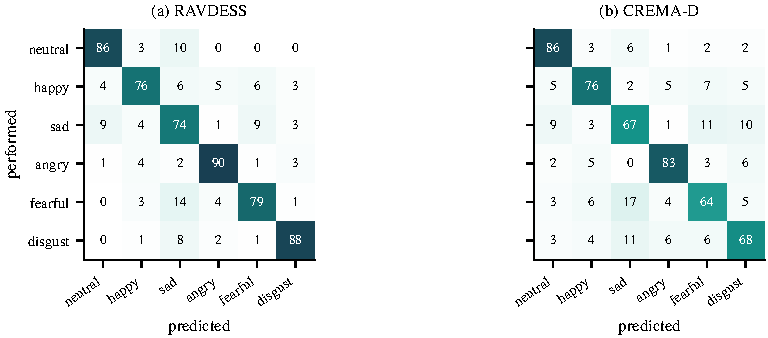
\includegraphics[width=0.85\textwidth]{fig_confusion}
\caption{Row-normalised confusion matrices (\%) of the best model, out-of-fold on unseen speakers.}
\label{fig:cm}
\end{figure*}

\subsection{Class separability}
In the raw feature spaces, clips hardly group by emotion. The cosine silhouette score using emotion labels is $-0.05$ for eGeMAPS and $0.01$ for WavLM on RAVDESS ($-0.03$ and $-0.01$ on CREMA-D). Most of the variation in the features comes from the speaker, the sentence and the recording, not from the emotion. A supervised projection gives a different picture. Fig.~\ref{fig:lda} shows a linear discriminant analysis of the combined features, fitted on folds 1--4 and then applied to fold~0. The unseen speakers land close to the training cluster of their emotion. Angry and disgust form clusters of their own, neutral and happy lie to one side, and sad and fearful overlap in the middle, which matches the confusions above. \clipA{} sits inside the angry cluster. Table~\ref{tab:pair} gives the speaker-independent ROC-AUC of a binary classifier for each pair of emotions. Every pair is above 0.89. The hardest pairs are sad--fearful (0.893) and sad--disgust (0.925) on CREMA-D and sad--fearful (0.946) on RAVDESS.

\begin{figure}[!t]
\centering
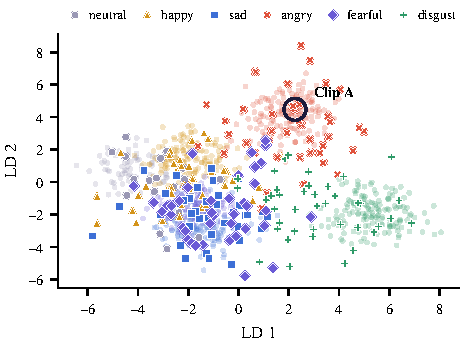
\includegraphics[width=\columnwidth]{fig_lda}
\caption{LDA map of the combined RAVDESS features. Faded points are the fold 1--4 speakers used to fit the map; solid markers are the unseen fold-0 speakers. The black circle marks \clipA{}.}
\label{fig:lda}
\end{figure}

\begin{table}[!t]
\centering
\caption{Pairwise separability: speaker-independent ROC-AUC of a binary LogReg on fused features. Upper triangle RAVDESS, lower triangle CREMA-D}
\label{tab:pair}
\footnotesize
\setlength{\tabcolsep}{3pt}
\begin{tabular}{@{}lcccccc@{}}
\toprule
 & neu & hap & sad & ang & fea & dis \\
\midrule
neu & -- & 0.983 & 0.970 & 0.996 & 0.999 & 1.000 \\
hap & 0.987 & -- & 0.968 & 0.981 & 0.978 & 0.996 \\
sad & 0.963 & 0.981 & -- & 0.990 & \textbf{0.946} & 0.973 \\
ang & 0.993 & 0.973 & 0.993 & -- & 0.982 & 0.989 \\
fea & 0.986 & 0.954 & \textbf{0.893} & 0.984 & -- & 0.995 \\
dis & 0.992 & 0.969 & \textbf{0.925} & 0.966 & 0.958 & -- \\
\bottomrule
\multicolumn{7}{@{}l}{\scriptsize Bold: AUC below 0.95.}
\end{tabular}
\end{table}


\subsection{Explaining a prediction: \clipA{}}
The demo model, trained without fold~0, gives \clipA{} 90.5\% angry and 9.1\% fearful. Fig.~\ref{fig:shap} shows the eight largest SHAP values the explainer assigns to \emph{angry}. A high alpha ratio, meaning more energy at high frequencies and a tense, bright voice, adds $+3.61$. A steep rise in loudness at word onsets adds $+2.11$ and high average loudness $+1.64$. Pulling the other way are a high first formant ($-2.26$) and MFCC~2 ($-2.17$). The 88 contributions add up exactly: $-0.18 + 2.86 = 2.68$. These directions fit what is known about the acoustics of anger~\cite{egemaps}. It should be noted that the named-feature explainer on its own would label \clipA{} fearful (54\%) rather than angry (7\%). The application reports such disagreements to the user rather than hiding them.

\begin{figure}[!t]
\centering
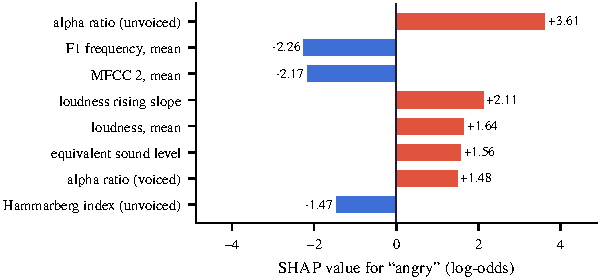
\includegraphics[width=\columnwidth]{fig_shap_clip_a}
\caption{Local explanation of \clipA{}: the eight largest exact SHAP values for ``angry'' from the eGeMAPS explainer. Red bars push towards angry, blue bars away from it.}
\label{fig:shap}
\end{figure}

\textbf{Global explanation.} Averaging $|\phi|$ over all out-of-fold clips shows that the CREMA-D model leans most on equivalent sound level, mean loudness and formant amplitudes, while the RAVDESS model leans on MFCC~1, first-formant frequency and spectral balance. Per feature, the energy group is the most informative in both corpora, as Dixit \emph{et al.}~\cite{dixit} also found. SHAP and permutation importance rank the features similarly (Spearman 0.79 on RAVDESS, 0.96 on CREMA-D). SHAP also revealed a preprocessing flaw that accuracy alone had hidden: some ratio features with a mean close to zero produced single contributions of up to $\pm$170 log-odds. Clipping the standardised values at $\pm$5 removed the problem.

\subsection{Cross-corpus transfer (H1)}
In Table~\ref{tab:cross} we train on one corpus and test on the other. Every model loses 20 to 35 points of UAR. When the scaler is fitted on the source corpus only, WavLM's relative drop is 6.1 points larger than eGeMAPS's when we train on RAVDESS, which supports H1. Trained on CREMA-D, however, WavLM's drop is 18.4 points \emph{smaller}. A likely explanation is that an encoder trained on 24 actors in a single studio picks up that studio, while one trained on 91 varied speakers learns cues that carry over. Standardising each corpus with its own statistics, which needs no target labels~\cite{schuller}, wins back 2 to 13 points. So H1 depends on the direction of transfer.

\begin{table}[!t]
\centering
\caption{Cross-corpus UAR (\%) with LogReg, with 95\% speaker-bootstrap intervals for the H1 gap. In-domain rows: mean over the five speaker folds}
\label{tab:cross}
\footnotesize
\setlength{\tabcolsep}{2.6pt}
\begin{tabular}{@{}llcccc@{}}
\toprule
\textbf{Direction} & \textbf{Scaling} & \textbf{eGeMAPS} & \textbf{WavLM} & \textbf{Fusion} & \textbf{H1 gap} \\
\midrule
R $\to$ C & source & 30.1 & 38.7 & 42.1 & $+6.1$ [3.1, 9.4] \\
R $\to$ C & per corpus & 35.6 & 45.0 & 48.6 & $+8.3$ [5.1, 11.6] \\
C $\to$ R & source & 30.0 & 58.8 & 66.3 & $-18.4$ [$-27.9$, $-8.1$] \\
C $\to$ R & per corpus & 43.2 & 67.8 & 68.3 & $-5.7$ [$-12.4$, 1.4] \\
\midrule
\multicolumn{2}{@{}l}{In-domain RAVDESS} & 55.4 & 81.0 & 82.2 & \\
\multicolumn{2}{@{}l}{In-domain CREMA-D} & 51.5 & 73.8 & 74.1 & \\
\bottomrule
\end{tabular}
\end{table}

\subsection{Stability of explanations (H2, H3)}
Fig.~\ref{fig:stab} compares the global SHAP rankings of pairs of models trained on different data. For the interpretable logistic regression, the median Spearman correlation falls from 0.78 between two resamples to 0.63 between two disjoint speaker groups and 0.50 between the two corpora, compared with 0.00 for random rankings, and every step is significant (Mann--Whitney $p<10^{-10}$). LightGBM and WavLM explanations are less stable, dropping to 0.20 and 0.10 across corpora. In other words, the most accurate representation has the least transferable explanation. Shares of whole feature groups turned out to be more stable than individual features. H2 is supported. Choosing a ``stable core'' of features instead of the top-$k$ most important ones gave one significant gain, four significant losses and seven results that were not significant across twelve settings, so H3 remains inconclusive.

\begin{figure}[!t]
\centering
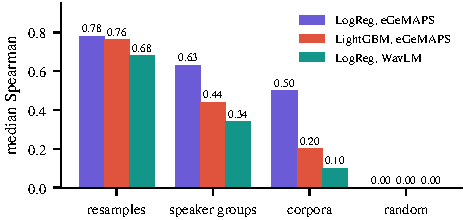
\includegraphics[width=\columnwidth]{fig_stability}
\caption{Median Spearman correlation between the global SHAP rankings of two models trained on two resamples, two disjoint speaker groups or two corpora, and between random rankings.}
\label{fig:stab}
\end{figure}

\subsection{Application}
The Streamlit app runs the saved pipeline on held-out dataset clips, uploaded files or microphone recordings. It shows the predicted emotion with all six scores, warns when the top two are within 15 points of each other, gives exact SHAP and ``why X and not Y'' explanations, and plots the waveform, energy and spectrogram of the cleaned signal. For real voices, the user can calibrate the model to their normal speaking voice and then record one sentence per emotion. In our tests on held-out speakers this short enrolment raised UAR in all ten settings, for example from 77.9 to 85.0\% on unseen RAVDESS speakers.

\subsection{Discussion and limitations}
The learned embeddings provide accuracy, while the named features provide reasons that a person can read; assigning each to its own role retains both benefits. Rigorous evaluation also matters: speaker leakage alone can add nine points. The main bottleneck is generalisation, which appears to depend more on how varied the training speakers are than on which features are used. Explanations deserve the same scrutiny as accuracy, because they shift across corpora too. The study has several limitations. Both corpora are acted English speech with intended rather than felt emotions, we study only one pair of corpora, the within-corpus models were trained with a single seed, and the microphone adaptations were tested on simulated rather than real recordings. The system recognises expressed emotion in short clips and should not be used to make decisions about people.

%=====================================================================
\section{Conclusion and Future Work}
%=====================================================================
Tested strictly on unseen speakers, logistic regression on combined eGeMAPS and WavLM features recognises six acted emotions with 82.2\% UAR on RAVDESS and 74.1\% on CREMA-D, is well calibrated, and can be explained exactly in terms of named voice properties. The analyses showed that the named features are highly redundant yet lose accuracy when compressed, that emotions are separable for a trained model even though raw distances barely reflect them, and that most errors involve quiet, low-energy emotions. Accuracy does not carry over well between corpora, and the explanations carry over only partly. Future work will add a third, non-acted corpus, probe WavLM's dimensions with eGeMAPS to give them names, evaluate domain-adversarial training for transfer, and use the CREMA-D listener ratings as soft labels.

\section*{Code and Data Availability}
Code, results and figures: \url{https://github.com/shreyashsp25/lucid-speech-emotion-xai}. RAVDESS: \url{https://zenodo.org/records/1188976}. CREMA-D: \url{https://github.com/CheyneyComputerScience/CREMA-D}. Every number in this report is produced by the notebooks and \texttt{src/} modules in the repository; the new analyses are in \texttt{src/review\_analysis.py} and the figures and tables in \texttt{report/ieee/}.

\bibliographystyle{IEEEtran}
\bibliography{refs}

\end{document}
